\documentclass[a4paper,10pt]{ltjsarticle}
\usepackage[haranoaji]{luatexja-preset}
\usepackage[margin=24mm]{geometry}
\usepackage{amsmath,amssymb,bm,booktabs,tabularx,graphicx}
\usepackage{enumitem,placeins,float}
\usepackage[round,authoryear]{natbib}
\usepackage{hyperref,url}
\hypersetup{hidelinks}
\setlength{\parindent}{1em}
\setlength{\parskip}{.2em}
\renewcommand{\arraystretch}{1.13}
\title{揃えた特化、異なる適応：\\共有表現における二次モーメント構造}
\author{匿名著者}
\date{日本語直訳版}
\newcommand{\figlang}{ja}
\newif\ifpublicrelease
\publicreleasefalse
\begin{document}
\maketitle
\begingroup
\renewcommand{\thefootnote}{*}
\footnotetext{生成AIが実験設計、実装、解析、文献調査、執筆を支援した。詳細はAI支援に関する声明に示す。}
\endgroup
\graphicspath{{../figures/}}
\begin{abstract}
% P:abstractnew
Adamで学習した小規模な共有表現ネットワークでは、選択した平均読み出し測定値が同等でも、同じ追加学習への応答は異なりうる。本研究は状態への介入によって二次モーメントの倍率と座標配置の効果を分け、その形成過程と時間依存性を調べる。中心となる二対象実験では、より精密に読み出せる対象が10更新以内に切り替わる割合は、取得経路で67.5\%、更新経路で0\%だった。一次モーメント交換による10更新の対比の変化は事前の判定幅内に留まる一方、二次モーメント交換は対比を反転させた。平均的な適応倍率を共通にしても配置の効果が残った。層別交換と移動量の制御は、全体の更新幅だけでは説明できない効果を特定した。形成中の記録は、小さいencoder二次モーメントと対象間の勾配の強い相殺を結びつけた。前向きの勾配射影実験はこの保持状態を変え、その二次モーメントだけを固定した学習器へ移すと10更新の適応応答が小さくなった。同等終点の比較は三Gaussian対象へ広がった一方、部屋のセンサ実験では成分効果が残っても終点一致は成立しなかった。検証した条件では、成分効果は反転や初期化同等性より広く成立した。効果の大きさと持続時間は学習条件に依存した。

\end{abstract}

\section{序論}
\label{sec:intro}
% P:introquestion
共有表現は複数の予測課題に使われる内部符号であり、容量が限られると、一部の対象が他より精密に読み出せることがある。本研究では、この読み出し精度の偏りを\emph{表現の特化}と呼ぶ。特徴の複雑さ、学習順序、情報源間の競合は、このような偏りを生みうる\citep{lampinen2024biased,pezeshki2021gradient,huang2022modality}。ここで問うのは、現在の特化を測れば、その変わりやすさも分かるかである。

% P:introstakes
評価後にモデルの学習を再開するとき、この問いは重要になる。現在の読み出し精度が近くても、同じ次の条件の下で共有特徴を再配分する応答は異なるかもしれない。学習履歴は重みと最適化器状態の両方を通じて、その後の学びやすさへ影響しうる\citep{achille2019critical,lyle2023plasticity,dohare2024plasticity}。そこで現在の測定能力と後の応答を分けて比較し、応答開始時の重みを固定したまま、保持された成分へ介入する。

% P:introcontribution
一方の対象を精密に観測する経路と、その対象の再構成誤差を重くする経路を用意する。調整用標本で校正し、別標本で選択した終点測定値の同等性を確認した後、共通の反対条件を与えると大きな初期応答差が現れた。本研究では、その測定値に隠れた応答差を\emph{潜在的感受性}と呼ぶ。本研究の貢献は、同等な読み出し測定値の下で二次モーメントの倍率と座標配置を分け、応答への効果をその形成過程へ結びつけた点にある。さらにモデル条件、三対象、長い継続学習を用いて、成分効果と、反転や初期化同等性が成立するより狭い条件を区別する。

\section{学習履歴・最適化器の記憶との関係}
\label{sec:related}
% P:related1
測定した性能が似ていても、予測器間に重要な違いが残ることは、過少特定の問題として研究されている\citep{damour2022underspecification}。表現類似度の測定は、終点の別の側面を調べる\citep{kornblith2019similarity}。本研究の比較対象は追加学習への応答であり、共通介入の前に選択した再構成測定値を揃える。この比較は、初期経験と学習過程が後の学習を変える可塑性研究につながる\citep{achille2019critical,jastrzebski2020breakeven,dohare2024plasticity}。

% P:related2
最適化器が媒介する履歴効果には、直接の先行研究がある。\citet{lyle2023plasticity}は可塑性を損失形状と関連づけ、課題変化後にAdamのモーメント推定が異なる速度で追随することが、学習を不安定にしうると示す。\citet{asadi2023resetting}は、強化学習の目的が変わった後の最適化器初期化を評価する。\citet{ellis2024local}は、勾配規模が変わった後の更新幅の過渡変化を解析し、相対的なAdam時刻を導入する。これらの結果から、引き継いだ適応倍率が、本研究で確かめる具体的な説明候補となる。問うのは、\emph{表現の再配分}における経路差を平均倍率で十分に説明できるか、それとも座標別配置も差を変えるかである。

% P:related3
隠れた学習効果を調べるために、状態を直接移植する研究もある。最近のプレプリントで\citet{xu2026optimizer}は、潜在的な特性転移を運ぶ一次モーメントを同定する。直後の出力に現れない介入が、その後の学習中に差を生む。\citet{sevetlidis2026trainingmemory}は履歴の保持先を整理し、状態に基づく因果的測定を提案する。本研究が加えるのは、共有表現の適応についての具体的な実証的分解である。再構成測定値の調整、二次モーメントの倍率・配置介入、引継ぎAdam・新規Adam・SGDでの共通継続を組み合わせる。最も近い比較を表\ref{tab:prior}にまとめる。

\begin{table}[t]
\centering\small
\caption{最も近い先行比較と、本研究で検証する問い。介入と測定結果を対応づけ、比較同士の関係を示す。}
\label{tab:prior}
\begin{tabularx}{\textwidth}{>{\raggedright\arraybackslash}p{.21\textwidth}>{\raggedright\arraybackslash}X>{\raggedright\arraybackslash}X}
\toprule
先行研究 & 確立された比較 & 本研究の比較\\
\midrule
\citet{lyle2023plasticity} & 変化する課題における可塑性、損失形状、最適化器の不安定性 & 選択した再構成測定値を揃えた後の再配分応答\\
\citet{asadi2023resetting,ellis2024local} & 状態・時刻の初期化と、目的・勾配規模変化による更新幅への影響 & 成分交換と、平均逆倍率を揃えた座標配置\\
\citet{xu2026optimizer} & 直後の出力不変性を含む、一次モーメント移植と後の転移 & 二次モーメント構造と特化応答の時間経過\\
\bottomrule
\end{tabularx}
\end{table}

\section{測定値を揃えた後の応答比較}
\label{sec:design}
\subsection{一つの共有ボトルネックを通る二つの形成経路}
% P:design1
中心となる学習器は、雑音を含む観測から二つの三次元信号$A$と$B$を再構成する。標準ガウス分布から$A$と独立な$\epsilon$を生成し、$\rho=0.35$として$B=\rho A+\sqrt{1-\rho^2}\epsilon$とする。seedごとの直交変換で観測を混合する。各層の後にtanhを置いた$6\to32\to2$エンコーダが、観測を二つの数値からなる符号へ写し、二つの線形再構成ヘッドがそれを共有する。学習対象は雑音のない信号である。このボトルネックにより、読み出せる情報の配分を観測できる。

% P:design2
情報品質と誤差の重みづけを別々に操作する。\emph{取得精度}は混合前の対象別入力雑音を変え、高精度・低精度の標準偏差は0.05と1.20である。各雑音チャネルを$\sqrt{1+\sigma^2}$で割り、分散を正規化する。\emph{更新配分}は再構成損失の重みを変える。
\begin{equation}
L_t=w_{A,t}\ell_{A,t}+w_{B,t}\ell_{B,t},\qquad w_{A,t}+w_{B,t}=1.
\label{eq:loss}
\end{equation}
重みを等しくすると、誤差の明示的な重要度は等しくなるが、勾配は異なりうる。したがって、観測品質は損失重みとは異なる介入を通じて学習へ入る。関連研究は能動的取得と課題重みづけを扱う\citep{shim2018joint,chen2022active,chen2018gradnorm,yu2020gradient}。本設計は、一つの共有表現でこれらの制御を交差させる。

% P:design3
均衡した100初期化更新の後、各経路で500更新を行う。均衡取得は、各対象に高精度更新を正確に250回ずつ割り当てる。終点を揃える比較では、取得経路は等損失重みで優位対象を精密に観測し、更新経路は取得を均衡させ、優位対象に重み0.80を与える。経路強度はパイロットseedで校正し、確認実験では固定する。測定と判定規則は\ref{app:measurement}に示す。

\subsection{共通測定と対応づけた推論}
% P:design4
読み出せる情報を測るため、エンコーダを固定し、未使用プローブデータで新しい線形読み出し器を当てはめ、別の未使用データで評価する。両対象に共通の高精度入力を与える。分散で正規化した平均二乗誤差を$D_A,D_B$とする。配分指数
\begin{equation}
s=\frac{D_B-D_A}{D_A+D_B}
\label{eq:s}
\end{equation}
は、$A$をより精密に読み出せるとき正になる。元の優位対象へ符号を揃えると、その低下が他方への再配分を測り、ゼロ交差は読み出しやすい対象の入れ替わりを示す。両誤差、その和、共通低精度プローブ下の配分も保持する。したがって、相対的な優位を絶対的な再構成品質とともに評価する。

% P:design5
各seedで共通の起点と対応づけた入力・雑音系列を用意する。条件は同じ初期モデルから分岐し、操作しない限り最適化器状態も共通とする。パイロットと確認seedは重複せず、各主要比較に40確認seedを用いる。推論では鏡像の対象ラベルをseed内で平均し、95\% seedブートストラップ区間を報告する。終点の同等性は、対応差の平均の区間が各事前許容幅内に入ることを要求するもので、全ペアの測定値が同一という主張ではない。全確認seedを保持する。形成後のモデルパラメータと表現の幾何形状は異なりうる。

% P:design7
各計画では、確認実行前に、配分指数または正規化誤差の単位で許容する平均差の上限を固定する。\ref{app:measurement}に、測定値を揃える許容幅と応答の同等幅、および別に設けたパイロット段階を示す。

\section{同程度の特化に隠れた応答差}
\label{sec:latent}
% P:response1
取得だけでも優位対象は変わる。等損失重みで$A$または$B$を精密に観測すると、独立した40確認seedの平均$s$は0.3385または$-0.3338$となった（図\ref{fig:headline}a）。二つの形成経路は、測定上似た特化へ到達する。符号を揃えた$s$、対象・非対象誤差、総誤差、低精度の符号を揃えた$s$という五つの終点基準をすべて通過する。符号を揃えた$s$の平均差は$-0.0064$（$[-0.0098,-0.0032]$）で、$\pm0.02$内にある。均衡観測・等重みの中立継続200更新にわたる平均積分応答も、引継ぎAdamと新規Adamのどちらでも同等である。したがって、選択した静的測定値と一つの中立継続要約を揃えたうえで、反対条件への応答を検証できる。

% P:response2
各形成済み学習器を、10更新からなる三つの反対介入へ複製する。取得だけのパルスは、等損失重みで、それまで読みにくかった対象を精密に観測する。更新だけのパルスは取得を均衡させ、その対象へ重み0.80を与える。複合パルスは、その対象を精密に観測して重み0.85を与える。各パルスを引継ぎAdamと新規初期化Adamで検証し、分岐時の受容側モデル重みは固定する。応答は符号を揃えた$s$の低下量、経路対比は取得形成の低下量から更新形成の低下量を引いた値である。

\begin{figure}[t]
\centering
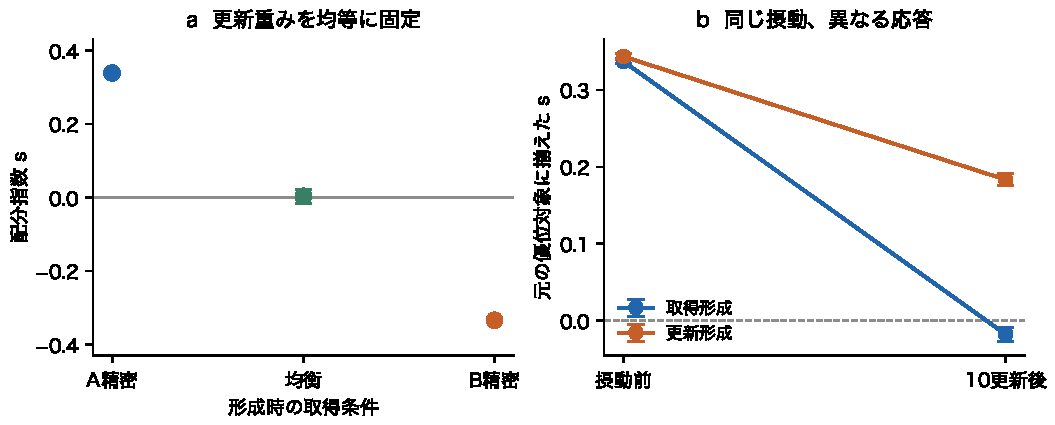
\includegraphics[width=.88\textwidth]{../figures/headline_ja.pdf}
\caption{共通の測定配分の背後に、異なる適応が隠れうる。(a) 等損失重みで取得が特化を選ぶ。(b) 終点を揃えた形成経路に、同じ複合反対パルスを与える。両者とも反対対象へ動くが、取得形成経路の変化が大きい。点と区間は40 seedを要約し、(b)の鏡像ラベルはseed内で平均する。線は途中の軌道ではなく、終点を結ぶ。}
\label{fig:headline}
\end{figure}

% P:response3
Adamを引き継ぐと、すべてのパルスで取得形成経路の変化が大きい（表\ref{tab:pulses}）。複合パルスでは、そのcheckpointの67.5\%が10更新以内にゼロを越えるのに対し、更新形成では0\%である（図\ref{fig:headline}b）。連続的な経路差は0.1951である。Adamを初期化すると0.0103へ減り、事前の$\pm0.02$幅内に入る。他のパルスでも同様に減少する。したがって、引き継いだ最適化器状態は、選択した終点測定と中立継続には現れなかった応答差を大きく変える。

\begin{table}[t]
\centering\small
\caption{反対条件10更新後の特化低下量の経路差。角括弧は95\% seedブートストラップ区間を示す。引継ぎ条件の全区間は$+0.05$より上、初期化条件の全区間は$\pm0.02$内にあり、それぞれの事前基準を満たす。}
\label{tab:pulses}
\begin{tabular}{lcc}
\toprule
パルス & Adam引継ぎ & Adam初期化\\
\midrule
取得のみ & $0.1668\ [0.1601,0.1736]$ & $0.0011\ [-0.0010,0.0035]$\\
更新のみ & $0.1510\ [0.1456,0.1562]$ & $0.0120\ [0.0093,0.0149]$\\
複合 & $0.1951\ [0.1880,0.2021]$ & $0.0103\ [0.0079,0.0129]$\\
\bottomrule
\end{tabular}
\end{table}

% P:response4
この結果は、二対象ネットワークと10更新パルスに適用される。別途測定した線形な表現類似度（CKA）の平均は0.927であり、モデルパラメータは同一ではない。Adamを初期化しても、これらのモデル差は残る。したがって小さな初期化対比が示すのは、この時間での限定された応答同等性であり、表現の同一性ではない。ゼロ交差率も短いパルスを記述する。第\ref{sec:time}節で、より長い共通学習を調べる。

\section{保持された状態が適応を変える仕組み}
\label{sec:mechanism}
\subsection{成分交換による二次モーメント効果の特定}
% P:mechanism1
Adamは、符号付き勾配の平均$m$と、勾配の二乗の平均$v$を保持する\citep{kingma2015adam}。後者はパラメータごとの適応倍率を定める。これらを直接検証するため、受容側の重みと最適化器の更新回数を固定し、経路終点間で$m$または$v$を交換する。両経路は同じ起点から分岐しているため、パラメータ座標を対応づけられる。

% P:mechanism2
独立した40 seed比較では、$m$交換による平均応答対比の変化は小さく、事前許容幅内にある。$v$を交換すると、経路対比は$+0.1968$から$-0.1265$へ変わる（図\ref{fig:moments}a）。両推定値の区間は、互いに反対側でゼロを除く（\ref{app:optimizer}）。したがって、受容側の二次モーメント状態は、どちらの経路が変化しやすいかを変える。この介入が同定するのは、受容側の重みと後続の勾配とともに働く因果的な修飾要因であり、測定対象は複合パルス10更新の応答である。

% P:mechanism5
経路内対照では、取得、ミニバッチ、更新回数、平均対象損失重みを固定する。一方は500更新を通じて重み0.80を使い、他方は1.00と0.60を無作為順に各250更新使う。終点基準は再び通過する。共通パルスでは、一定系列の変化が0.0324（$[0.0294,0.0354]$）大きい。$v$交換によって対比は$-0.0141$へ逆転し、Adam初期化では0.0046へ減って$\pm0.01$内に入る（図\ref{fig:moments}b）。したがって、取得形成と更新形成というラベルの違いは、この応答パターンに必要ではない。平均損失重みが等しくても、異なる最適化器状態と後の応答が隠れうる。この対照では、ばらつきと実現系列が同時に変わる。

\begin{figure}[t]
\centering
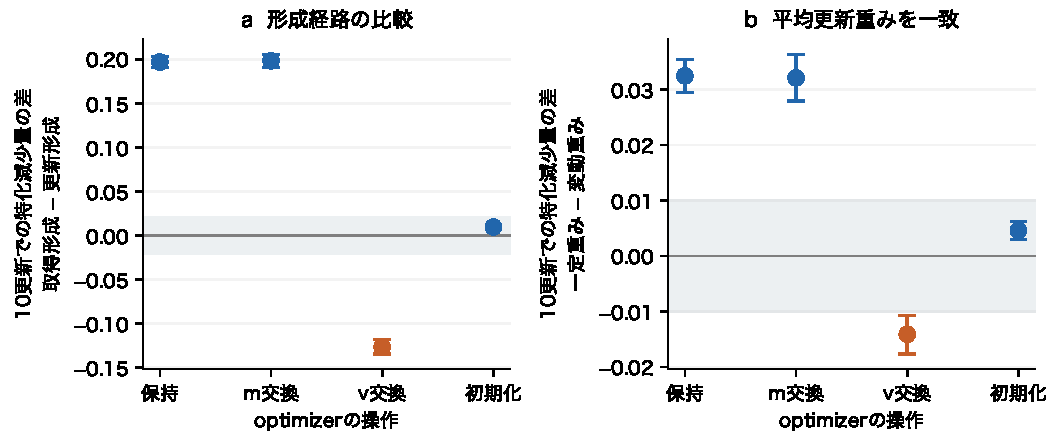
\includegraphics[width=.88\textwidth]{../figures/moments_ja.pdf}
\caption{二次モーメント交換は、二つの短時間応答対比を逆転させる。(a) 取得形成から更新形成を引いた特化低下量。(b) 取得と平均損失重みを固定した、一定から変動の重み履歴を引いた対比。帯は各事前同等性幅（$\pm0.02$、$\pm0.01$）を示す。区間は対応seedブートストラップで、各比較は重複しない40確認seedを用いる。}
\label{fig:moments}
\end{figure}

\subsection{倍率・所在・移動量}
% P:mechanism3
交換結果から、より具体的な問いが生じる。一方の経路は、単に平均的な適応倍率が大きいだけなのだろうか。新規40 seedの事前固定追試では、引継ぎ状態の対比は0.1907となり、先の推定値0.1951と0.1968が再現する。Adamのバイアス補正済み二次モーメント逆倍率を、パラメータ間で平均した量を$\bar a_v$と定義する。これは$v$が与える倍率であり、実際の更新は一次モーメントと現在勾配も利用する。

% P:mechanism4
各経路の座標配置を保ちながら$\bar a_v$を揃えると、応答差は0.1907から0.0875へ減る。配置を一つのスカラー値に置き換えると0.1251、スカラー化と共通倍率を組み合わせると0.0395となる（図\ref{fig:timecourse}a）。$\bar a_v$を共通に保って他経路の配置へ交換すると、差は$-0.0110$へ変わる。したがって、平均倍率は応答対比の一部を説明し、その共通平均の下でも座標配置が受容側の応答を変える。この比較で揃えるのは平均逆倍率であり、パルス全体の実際の更新ノルムではない。

% P:mechanism8
全体の経路長の違いだけで対比を説明できるか、移動量を制御して確かめた。各更新で四分岐（二経路、元または交換した$v$）の提案更新ノルムの幾何平均を共通目標とし、方向を保って大きさを揃える。元の$v$では対比が0.1907から0.0303へ、この規則の下で約84\%縮小した。交換した$v$では0.0072となり、対応する交換効果0.0231が残った。これは学習則を変更した比較での縮小率であり、自然なAdamの応答に対する移動量の因果的な媒介割合ではない。残った交換効果は、全体の移動量が等しくても再配分が異なりうることを示す（表~\ref{tab:ivfmechanism}）。

% P:mechanism9
適応倍率が置かれる場所は、$v$総量に占める割合以上に重要だった。取得形成checkpointでは、第1 encoder層は$v$総量の5.9\%しか持たないが、その層の交換で対比は0.1907から0.0115へ減った。headは66.2\%を持つが、その$v$を交換しても対比は0.1911だった。第2層の交換では0.0611が残った（表~\ref{tab:ivfmechanism}）。受容側の重みと他の最適化器成分は保持する。これらは有効な介入先をencoderに特定する結果であり、非加法的な効果を層ごとの独立な因果寄与率へ分解することはできない。

\subsection{勾配の衝突から保持状態への形成過程}
\label{sec:forming}
% P:formationstory
取得経路のencoder二次モーメントは、なぜ小さいのか。元の500更新の形成過程を記録して再実行すると、保存済み160終点すべてが厳密に再現された。二対象からの勾配はしばしば逆向きになり、その負の交差項は、重み付き個別二乗項の累積和の94\%と93\%を二つのencoder層で相殺した。更新経路では28\%と25\%だった。個別二乗項の和自体は取得経路のほうが大きかった。したがって、小さい二次モーメントには相殺と、均衡した祖先から残る大きな寄与が関わっていた。この分解は実際に変化する重みと入力に沿った記録である（付録~\ref{app:formationlogs}）。

% P:projectionmain
次に、共有encoderの二対象勾配へPCGrad射影を適用して形成を変えた\citep{yu2020gradient}。重み付き勾配が衝突すると、それぞれから相手と逆向きの成分を射影で除き、headの更新式は維持する。局所固定した計画で未使用40 seedを用い、元の取得経路と更新経路を対照として保持した。射影後の取得経路では、encoderの最終二次モーメント総和は元の$1.423\;[1.386,1.459]$倍、平均逆倍率は$0.713\;[0.705,0.721]$倍となった。この履歴の$v$だけを元の取得経路の学習器へ移すと、10更新の応答は$-0.0472\;[-0.0489,-0.0455]$だけ変化し、小さくなった（図~\ref{fig:projection}）。

% P:projectionmagnitude
射影は個々の勾配を縮める一方、相殺を減らして合成勾配の二乗ノルムを増やしたが、最終$v$は更新経路を下回った（図\ref{fig:projection}a）。大きさと相互作用が同時に変わるため、元の状態差を相殺と観測品質の寄与へ分割することはできない。

% P:projectioninterpret
交差移植は、各学習器を固定して$v$を変える。どちらも射影履歴の$v$では10更新の応答が小さくなった。射影は重みと$m$も変え、終点一致を満たさなかったため、その総効果は同等終点での再現や自然な媒介割合を与えない。この実験が示すのは、形成を変えて作られた異なる$v$だけで、固定した学習器の応答が変わることである。50更新では供与効果は小さな正の値になった。交差比較、未達基準、副次的な時間幅を付録~\ref{app:projection}に示す。

\begin{figure}[t]\centering
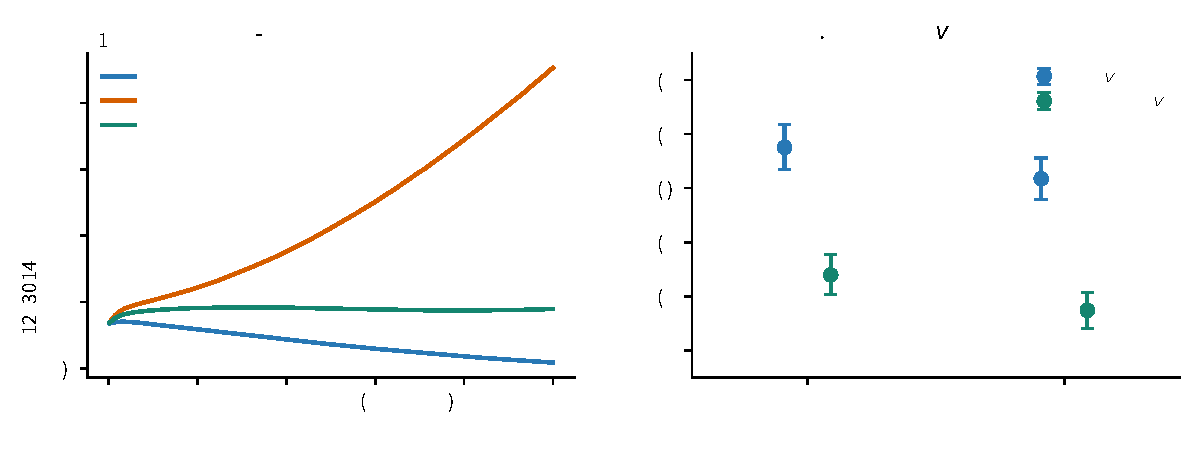
\includegraphics[width=.94\textwidth]{../figures/projection_ja.pdf}
\caption{形成への介入と学習器を固定した比較。(a) 未使用40 seedでの形成中のencoder二次モーメント総和。(b) 元の取得経路と射影後の取得経路それぞれに、元または射影履歴の二次モーメントを与えた10更新の特化減少。同じ学習器内ではpulse開始前の重み・一次モーメント・更新時刻を固定し、$v$だけを変える。誤差棒はseed対応bootstrapの95\%区間。}
\label{fig:projection}
\end{figure}

\section{効果の時間幅と成立範囲}
\label{sec:time}
% P:time1
初期化直後の差が小さくても、学習の継続中に大きくなる可能性がある。そこで反対介入を、引継ぎAdam、新規Adam、モーメンタムなしSGDで500更新まで延ばす。SGDの共通学習率は、seed・対象方向ごとに、最初のバッチの引継ぎAdam更新ノルムと勾配ノルムを使って校正し、以後固定する。配分応答は校正に使わない。三つの継続はいずれも、Adamで形成した経路終点から始める。

% P:time2
引継ぎAdamの経路差は10--20更新で最大となる。新規Adamは10更新の0.0096から50更新の0.0274へ、校正SGDは10更新の0.0123から50更新の0.0433、100更新の0.0309へ変わる（図\ref{fig:timecourse}b）。50更新の新規AdamとSGDの区間は0.02より上にある。この幅は10更新検証で固定したもので、後の時点では参照に用いる。観測結果は、引き継いだAdam状態を除いた後にも経路差が遅れて現れることを示し、モデル側に残る差の関与を示すが、特定のパラメータや幾何学的な原因は同定しない。

% P:time3
経路対比は500更新までにゼロへ近づく。引継ぎAdamの配分終点差は$-0.00045$（$[-0.00146,0.00057]$）である。開始測定値は近いが同一ではないため、この終点差は形成からの変化量の差とは別の量である。また、引継ぎから新規Adamを引いた応答対比は50更新までに符号を変える。そのため、新規Adamの軌道へ固定した非負の高速成分を足すだけでは、引継ぎ軌道を記述できない。この共通反対条件の範囲では、最適化器状態が再配分の時期と大きさを変え、大きな初期差が持続的な配分差を意味するわけではない。

\begin{figure}[t]
\centering
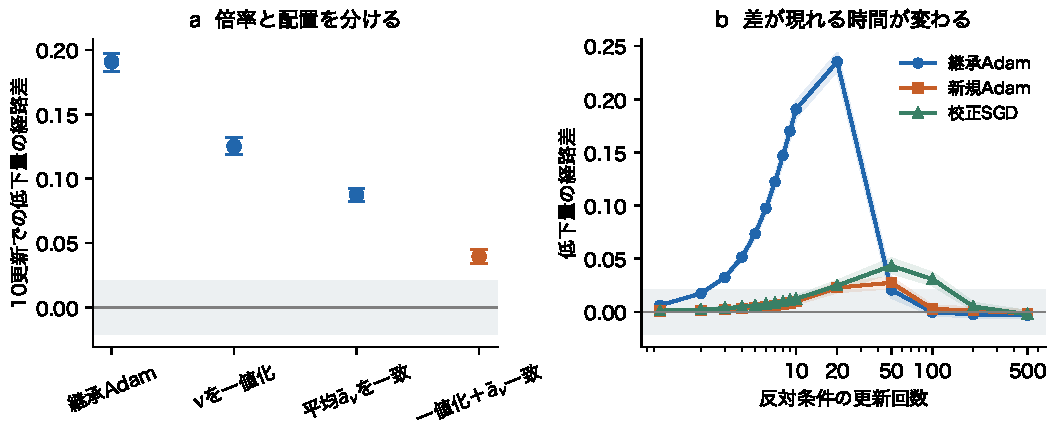
\includegraphics[width=.88\textwidth]{../figures/timecourse_ja.pdf}
\caption{倍率・配置介入と観測時間は、応答の異なる部分を明らかにする。(a) 引継ぎ状態、$v$のスカラー化、$\bar a_v$の統一、または両方の介入後の10更新経路対比。(b) 引継ぎAdam、新規Adam、校正SGDで反対条件を共通に継続する。$\pm0.02$の帯は10更新の同等性幅であり、後の時点にはこの幅による事前判定規則はない。平均と95\%対応seedブートストラップ区間は新規40 seedを用いる。}
\label{fig:timecourse}
\end{figure}

% P:generalization
IV-Fでは新しい32対応seedを用い、中間層幅、活性化関数、対象相関、二次モーメントの減衰率、形成時間を変えて比較した。重複しない九設定はすべて五つの終点許容幅を満たし、共通倍率での配置効果が正だった（表~\ref{tab:claims}）。この効果は、共通$\bar a_v$での自己配置の経路対比から、交換配置の経路対比を引いた量である。反転と初期化同等性が成立する設定は、これより少なかった。例えば幅64では反転が残る一方、初期化後の区間全体が0.02より上にあった。したがって、成分効果は、これら二つのより強い応答パターンより広い範囲へ移った。

% P:durationnew
形成を長くしても、倍率は一律には変化しない。調べたすべての$\beta_2$で、自己状態の応答差は500更新より1,500更新で大きく、1,500更新の初期化後区間はすべて0.02を超えた。$\beta_2=0.9$では両期間とも初期化が差を増やした。保持状態は経路差を弱める場合もある。保存checkpointでは、取得／更新の平均逆倍率比は0.999で期間とともに増えた一方、0.9と0.99では減った。したがって、500更新で観察した相殺機構から、倍率比が一律に拡大するという説明で格子全体を説明することはできない（\ref{app:extension}）。

% P:vbmain
成分効果は、代替対象が一つしかないことに依存するだろうか。対称な三つのGaussian対象について取得・更新による履歴を形成し、優先対象を変える六つの順序付き方向を調べた。8パイロットseedでは適応を観測せず終点測定だけで校正し、新規40 seedで容量2と3を検証した。応答は、元の対象と移行先との二対象配分指数の低下量とし、三対象すべての誤差を保存した。両容量で八つすべての平均終点基準を満たした。$v$交換は10更新の経路対比を反転し、共通$\bar a_v$での配置交換も両容量で対比を変えた（表~\ref{tab:claims}、\ref{tab:vb}）。初期化後の同等性は容量2で成立したが、容量3では区間が$+0.02$をまたいで未解決だった（付録~\ref{app:threeadapt}）。

% P:naturalnew
部屋のセンサへの拡張は、制御された再構成課題を維持したまま、実測値の不均一な分布を調べる。各室の温度と湿度を使えば、三つの二変数対象として、介入を設計し直さずGaussian対象を置き換えられる\citep{candanedo2017data,candanedo2017dataset}。両容量で共通倍率の配置効果が残った一方、独立確認では終点一致が成立しなかった（表~\ref{tab:claims}）。これは入力分布を変えても成分効果が残る証拠であり、実測データで同等終点に応答差が隠れることの実証には至っていない。一住宅の固定した時刻ブロックを用いたため、住宅間や異なる課題への一般化も未検証である（付録~\ref{app:natural}）。

\begin{table}[t]
\centering\small
\caption{拡張13設定における10更新の帰結。Yは基準成立、Nは区間が不成立を示す、?は判定未確定。終点一致は全測定区間が許容幅内、共通倍率での配置効果は区間が正、反転は元が正で$v$交換後が負、初期化同等は区間が$\pm0.02$内であることを要する。個別の95\%区間を用い、設定の母集団に対する成功率は推定しない。IV-Fは共通32 seed、V-BとV-Cはそれぞれ40 seedを容量間で共有する。基準設定は一度だけ数える。ここでの反転は符号の基準であり、自己対比の区間下限が$+0.05$を超えるという別の事前基準は、室内センサの容量2では未達だった。}
\label{tab:claims}
% P:claimstable
\begin{tabular}{lcccc}
\toprule
設定 & 終点一致 & \shortstack{共通倍率での\\配置効果} & 反転 & 初期化同等\\
\midrule
基準 ($\beta_2=0.999$, 500) & Y & Y & Y & Y\\
幅64 & Y & Y & Y & N\\
ReLU & Y & Y & Y & Y\\
$\rho=0$ & Y & Y & Y & Y\\
$\beta_2=0.9$, 500 & Y & Y & N & N\\
$\beta_2=0.99$, 500 & Y & Y & Y & Y\\
$\beta_2=0.9$, 1500 & Y & Y & N & N\\
$\beta_2=0.99$, 1500 & Y & Y & N & N\\
$\beta_2=0.999$, 1500 & Y & Y & Y & N\\
Gaussian, $d_Z=2$ & Y & Y & Y & Y\\
Gaussian, $d_Z=3$ & Y & Y & Y & ?\\
実測センサ, $d_Z=2$ & N & Y & Y & Y\\
実測センサ, $d_Z=3$ & N & Y & ? & Y\\
\bottomrule
\end{tabular}
\end{table}

\section{含意}
\label{sec:scope}
% P:scope1
この結果は、継続学習を検証する具体的な方法を与える。現在の特化を測り、同じ将来学習条件を加え、どの持続状態成分が応答を変えるかを調べる。本構成では、平均再構成測定値が同等でも大きな初期対比が生じ、$v$交換によって逆転する。平均的な適応倍率が説明するのは、その対比の一部である。さらに、平均損失重みを揃えた対照は、課題の平均的な重視度が同じでも、保持状態と応答が異なりうることを示す。これらの比較は、最適化器の記憶を、共有表現内の情報再配分と結びつける。

% P:scope2
具体的な応用場面は、課題を変えて学習を再開する前のチェックポイント評価である。この比較から、現在の読み出し品質に加え、最適化器状態を引き継ぐ場合と初期化する場合に、共通の継続学習を試す方法が考えられる。本実験系では、この選択によって適応の時期と大きさが変わる。同じ診断がファインチューニングの判断に役立つかは、最終的な性能を含め、対象課題で検証する必要がある。

% P:scopecompact
同等終点の証拠が対象とするのは、小規模bottleneckネットワーク、二つまたは三つのGaussian対象、指定した観測・損失履歴、有限の継続期間である。選択した平均読み出しを揃えても、モデルの全機能や幾何構造を揃えたことにはならない。成分介入では分岐点の学習器を固定して比較し、共通祖先から対応する座標へ移植する。実用的なcheckpoint選択に使えるかは、再配分の速さをそのまま良さとみなさず、最終性能を含む対象課題の証拠で確かめる必要がある。

\section{結論}
% P:conclusion
検証した二・三対象のGaussian系では、測定した特化が近くても追加学習への潜在的感受性が異なりうる。成分交換は、引き継いだAdamの二次モーメントが初期再配分を因果的に変えることを示した。平均適応倍率を揃えても、二対象対照では全体の更新ノルムを揃えても、効果が残った。形成記録と射影後の移植は、学習中の勾配を、受容側の応答を変える二次モーメントへ結びつけた。実測センサ拡張でも成分効果は残ったが、終点一致は満たさず、介入効果の移植と隠れた応答差の実証を区別する結果となった。初期化同等性と符号反転は、容量、学習条件、観測時間に依存する。現在の読み出し品質、保持された学習状態、その後の条件が、適応の比較で現れる差をともに決める。

\section*{再現性に関する声明}
% P:repro
\ifpublicrelease
コードと生成データは\url{https://github.com/culturegeek/matched-specialization-different-adaptation}（\href{https://github.com/culturegeek/matched-specialization-different-adaptation/releases/tag/v1.5.2}{v1.5.2}）から入手できる。
\else
本稿には、匿名化したコードとデータのアーカイブを補足資料として添付する。
\fi
アーカイブには、本稿で報告した研究と、それを含む研究全体のソースコード、ローカルで固定した計画、seed別軌道、チェックポイント、監査スクリプトを含む。コードはMIT、生成データと説明資料はCC BY 4.0で提供する。再配布するUCIセンサデータは、元のCC BY 4.0の出典表示を保持する。\ref{app:status}で主張とファイルを対応づけ、CPU上での完全性・数値・図生成・学習再現の検査を示す。

\section*{広範な影響に関する声明}
% P:impact
本研究は、入力へのアクセスと学習履歴が時間とともに変わる共有表現を調べるための制御比較を提供する。運用中のシステムへ適用するには、その環境で介入と測定を直接検証する必要がある。

\section*{AI支援に関する声明}
% P:ai
生成AIシステムを、多くの実験設計と追試解析の提案、実装と実行、出力の解析、文献調査、原稿の執筆と翻訳に広く使用した。人間の著者は、研究全体を発案し、この実証研究を依頼し、主要な判断時点で継続を承認し、証拠と主張を確認し、論文とその公開について責任を負う。

\bibliography{references}
\bibliographystyle{tmlr}
\FloatBarrier
\appendix
\section{測定と対応のある推論}
\label{app:measurement}
% P:measurementcompact
中心ネットワークは$6\to32\to2$で、encoderの各層の後にtanhを置く。二つの線形headがこのencoderを共有する。学習・probe・test標本数は$3072/768/1536$、batchは256、Adam学習率0.002、$(\beta_1,\beta_2)=(0.9,0.999)$、$\epsilon=10^{-8}$、weight decay $10^{-5}$、読み出しridge係数$10^{-3}$である。seedごとに共通祖先、対応するデータとbatchを用いる。新たな線形読み出し器を未使用probeで学習し、別testで評価する。共通の高精度・低精度入力を用いて、学習された読み出し精度と、その時点の観測精度を区別する。

% P:appmargins
形成の許容幅は、符号を揃えた$s$、対象・非対象誤差とその和で$\pm0.02$、低精度の符号を揃えた$s$で$\pm0.01$である。IV-Dは、応答の判定幅として、中立継続と初期化後応答に$\pm0.02$、引継ぎ状態のパルスに$\pm0.05$を用いる。IV-Eは$m$交換による変化と初期化後応答に$\pm0.02$、経路内の更新履歴対照は初期化後応答に$\pm0.01$を用いる。これらの基準を、対応差の平均の区間へ適用する。

% P:appmarginrule
IV-Dでは、95\%区間全体が指定幅の内側に入れば同等、正負いずれかの境界の外側に完全に出れば実質差あり、それ以外は未解決と判定する。引継ぎ条件の三つのパルス区間は、いずれも全体が$+0.05$より上にあり（表\ref{tab:pulses}）、正の実質的な経路差を示す。初期化条件の全パルス区間は$\pm0.02$内に入る。

% P:appmarginorigin
IV-Dはパイロットseed 8000--8015で経路強度を校正し、seed 8100--8139の前に許容幅を固定する。IV-Eはパイロットseed 9000--9015を用いて応答基準を定め、その後にseed 9100--9139を実行する。経路内対照は、パイロットseed 9200--9215を応答基準と同等幅の設定に明示的に用い、その後にseed 9300--9339を実行する。計画にはこれらの操作上の選択が記録されているが、独立した実用誤差の基準から許容幅を導いてはいない。したがって、同等性は、これらの人工的な比較で明示した分解能における一致を表す。

% P:endpointpredictioncompact
終点同等性は選択した測定値のseed内平均差の区間に関するもので、すべてのseed対やモデルの全機能の一致ではない。表現類似度CKAの平均は0.927だった。保存データでは、対象誤差、他対象誤差、低精度配分の経路差から10更新の応答差を予測した。seedを一つずつ除外した評価で、学習側平均だけの予測に対する二乗誤差比は、独立した三つの40-seed標本で1.118、1.023、0.984だった。測定した残差特徴による線形予測の改善は小さく、未測定の幾何構造による交絡を除いたことにはならない。全予測値を保存している。

\section{状態介入と継続学習}
\label{app:optimizer}
% P:appopt1
IV-Dでは40確認seedと、seedごとの二つの鏡像方向を用いる。符号を揃えた平均$s$は、取得主導形成で0.3375、更新主導形成で0.3439である。対応する対象側・非対象側誤差は0.4034/0.8144と0.4000/0.8198である。経路強度はパイロットで校正しており、確認終点へ当てはめていない。中立継続の積分差は、Adam引継ぎで$-0.0025$（$[-0.0064,0.0013]$）、初期化後で$-0.0018$（$[-0.0068,0.0030]$）である。取得、更新、複合パルスにおける引継ぎと初期化の応答交互作用は0.1657、0.1390、0.1848であり、いずれも事前基準0.08を上回る。

% P:appopt2
IV-Eでは、自己状態から$m$交換を引いた変化は$-0.0014$（$[-0.0044,0.0018]$）で、$\pm0.02$内にある。取得形成経路の二次モーメント総量は更新形成経路の0.5577倍であり、座標別の二次モーメント逆スケーリング係数の平均は1.950倍である。この係数は実際のパラメータ更新量の比ではない。Adamの更新は、一次モーメント、現在勾配、バイアス補正にも依存する。主要成分比較を表\ref{tab:components}に示す。

\begin{table}[h]
\centering\small
\caption{成分介入下の複合パルス応答差。IV-Eは取得形成から更新形成を引いた比較、対照は一定から変動の更新重み履歴を引いた比較である。それぞれ重複しない40確認seedを用いる。}
\label{tab:components}
\begin{tabular}{lcc}
\toprule
成分条件 & IV-E経路差 & 平均を揃えた更新履歴対照\\
\midrule
自己の状態 & $0.1968\ [0.1910,0.2029]$ & $0.0324\ [0.0294,0.0354]$\\
$m$交換 & $0.1982\ [0.1912,0.2054]$ & $0.0321\ [0.0277,0.0362]$\\
$v$交換 & $-0.1265\ [-0.1348,-0.1183]$ & $-0.0141\ [-0.0176,-0.0110]$\\
初期化 & $0.0097\ [0.0078,0.0117]$ & $0.0046\ [0.0031,0.0062]$\\
\bottomrule
\end{tabular}
\end{table}

% P:withinroutecompact
平均重みを揃えた履歴対照では、優位対象の重みを一定の0.80とする条件と、1.00および0.60を各250更新、無作為順で使う条件を比較し、取得・batch・総更新数を固定した。調整と確認のseedは独立である。終点基準はすべて通過し、応答差を表~\ref{tab:components}に示す。ばらつきと順序は同時に変わる。この対照は、取得／更新という異なる経路ラベルがなくても効果が生じることを示し、順序だけの効果は未同定のまま残す。

% P:scaleprocedure
更新時刻$t$、パラメータ数$P$に対し、平均適応倍率を
\begin{equation}\bar a_v=P^{-1}\sum_j\frac{\eta}{\sqrt{v_j/(1-\beta_2^t)}+\epsilon}\end{equation}
とする。共通の目標値は二経路の元の値の幾何平均である。配置を保つ正規化では$v$を$cv$へ置き換え、$\epsilon$を含む80回の二分探索で正の$c$を求める。配置交換は$v$を移植した後に正規化する。スカラー化は共通または自己倍率$a_\ast$を用い、全座標を$v_j=(\eta/a_\ast-\epsilon)^2(1-\beta_2^t)$とする。学習器の重み、$m$、更新時刻を固定し、倍率の相対誤差は$2\times10^{-6}$未満である。共通祖先が対応する座標を与える。

% P:continuationcompact
追試はseed 20000--20039を用いた。momentumなしSGDでは、seed・方向ごとに、最初のbatchのAdam更新ノルムを正則化勾配ノルムで割った二経路の値の幾何平均を共通学習率とし、以後固定した（0.0194--0.0529）。応答測定値は校正に使わない。主評価の10更新の判定幅を、後の時刻の確認的判定へ流用しない。50更新のfresh AdamとSGDの応答差の区間は$[0.0227,0.0321]$、$[0.0368,0.0499]$である。500更新では測定した配分の終点が近づき、モデル全状態の収束は未検証である。別の10更新pulse後に中立継続する条件でも、終点差は50更新の0.06197から510更新の0.00984へ減少した。

\section{保持状態の所在・形成記録・介入}
\label{app:mechanism}
\subsection{層と移動量の対照}
\label{app:layers}
% P:movementprocedure
層別交換はbiasを含む指定層の$v$だけを変える。移動量の対照では、二経路の自己／交換$v$による四枝を同時に進め、各時点の提案更新のEuclideanノルムの幾何平均を共通ノルムとする。更新方向を保って再尺度化し、モーメントは実際の位置で更新を続ける。達成した相対誤差は$2\times10^{-6}$未満である。これらは学習則を変える介入であり、自然なAdamの媒介割合や層ごとの加法的寄与を同定しない。

\begin{table}[H]
\centering\small
\caption{保存済み40 seed対応組での層別・移動量介入。層の行は指定層の$v$だけを交換し、移動量統一の行は共同ノルム制御則を用いる。}
\label{tab:ivfmechanism}
% P:appfmechanismtable
\begin{tabular}{lr}
\toprule
介入 & 経路対比［95\%区間］\\
\midrule
元の状態 & $0.1907\;[0.1837,0.1976]$ \\
encoder第1層 & $0.0115\;[0.0060,0.0171]$ \\
encoder第2層 & $0.0611\;[0.0558,0.0665]$ \\
両head & $0.1911\;[0.1838,0.1978]$ \\
全パラメータ & $-0.1183\;[-0.1264,-0.1099]$ \\
移動量統一・元の$v$ & $0.0303\;[0.0269,0.0338]$ \\
移動量統一・$v$交換 & $0.0072\;[0.0040,0.0104]$ \\
\bottomrule
\end{tabular}

\end{table}

\subsection{形成履歴の分解}
\label{app:formationlogs}
\label{app:headgrad}
% P:loggingdesigncompact
探索的再実行では、元の追試の40 seed、両方向、両経路を保持し、入力、batch、損失重み、Adam設定を変えない。元の重み付きbackwardの前にhead別勾配を記録し、記録環境では160終点がbitwise一致した。$g_f,g_o$を重み付け前のhead勾配とすると、重み付き合成勾配の二乗は、個別二乗項、交差項、weight decay項へ分かれる。各項を同じ$\beta_2$で累積すれば、座標ごとに
\begin{equation}v_T=\beta_2^T v_0+S_T+C_T+R_T+E_T\end{equation}
となる。$S_T$は$w_f^2g_f^2+w_o^2g_o^2$、$C_T$は$2w_fw_og_fg_o$の累積で、$R_T$は結合weight decay、$E_T$は浮動小数点の残差である。相殺率は層内座標を足した後の$-C_T/S_T$とし、方向をseed内で平均する。これは観測された軌道の算術的分解である。

% P:formationlogresult
取得経路では形成を通じて平均的に打消しが強かった（図~\ref{fig:formationlogs}）。500更新後の$-C/S$は、第1・第2 encoder層で$0.942\;[0.939,0.945]$と$0.930\;[0.927,0.934]$であり、更新経路では$0.284\;[0.271,0.298]$と$0.252\;[0.238,0.268]$だった。最終$v$の取得／更新比は、それぞれ$0.242\;[0.230,0.255]$と$0.340\;[0.321,0.361]$だった。方向ごとの割合をseed内で平均すると、取得経路の最終$v$の約64\%と79\%は初期状態からの残存分で、更新経路では16\%と28\%だった。蓄積した個別二乗項の合計$S$の平均は、両層とも取得経路の方が大きかった。したがって、小さな最終状態には、新しく蓄積する課題勾配の強い相殺と、相当量の引継ぎ成分の両方が関わっていた。

% P:paireds
個別二乗和の経路差を、同じseed同士で対応させて評価した。取得−更新の$S_T$は第1層で$0.000931\;[0.000831,0.001035]$、第2層で$0.000355\;[0.000088,0.000636]$だった。両層の対応差の区間は正で、第2層の差は小さい。

% P:strata
観測条件別の集計は蓄積の所在を示す。第1層では、優位対象が常に精密な取得経路の平均cosは約$-0.94$、相殺率は0.94である。更新経路で優位対象が精密なstepは$-0.81$と0.48、他対象が精密なstepは約$-0.08$と0.06だった。251--500更新では後者の交差項が正に転じ（cos約$+0.11$、相殺率$-0.12$）、初期ピーク後に累積相殺率が減ることと整合する。これらは変化する状態と損失重みの下での条件付き観察であり、観測精度だけの因果効果ではない。

\begin{figure}[ht]
\centering
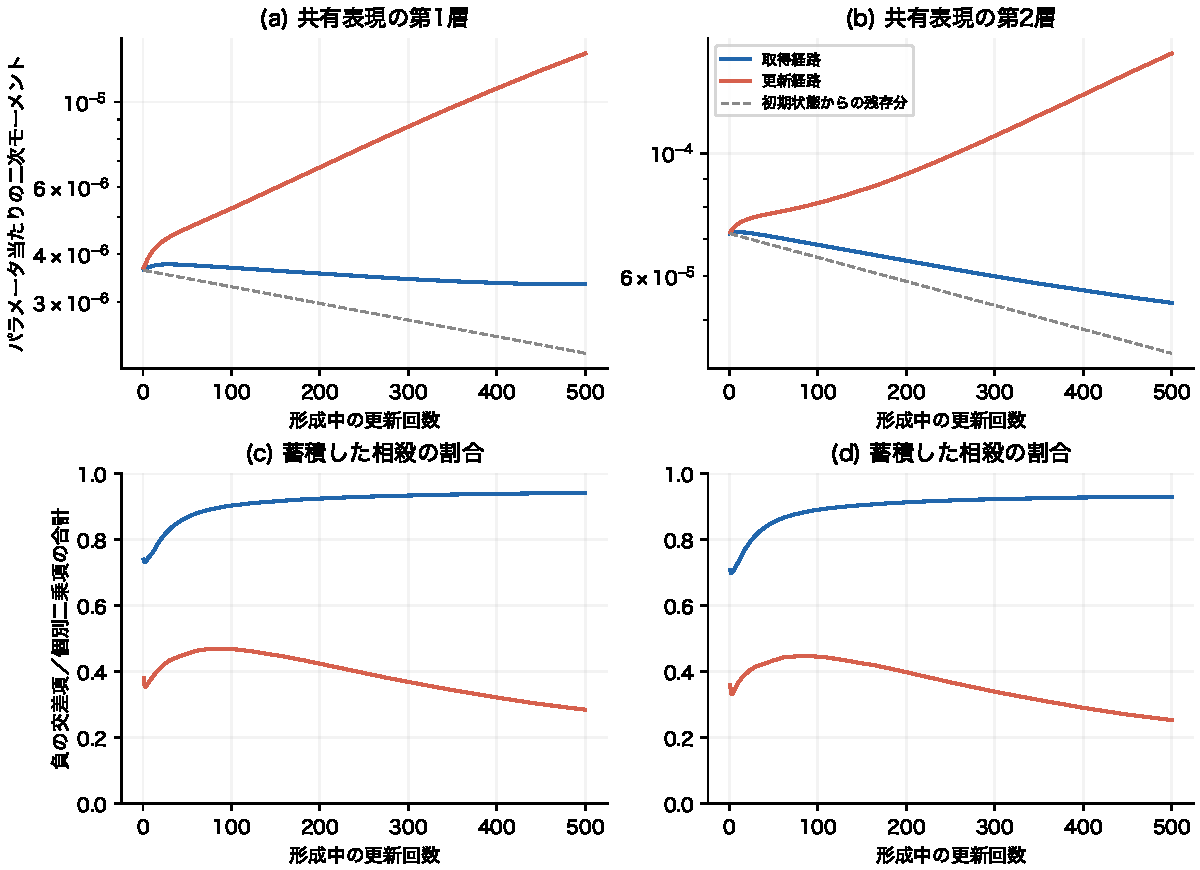
\includegraphics[width=.86\textwidth]{../figures/formation_logging_ja.pdf}
\caption{元の40対応seedによる形成中の分解。上段は各encoder層のパラメータ当たり二次モーメントの平均で、破線は共通の初期状態から減衰して残る量。下段は、各経路の実際の観測と損失重みの下で蓄積した相殺割合$-C/S$の平均。曲線は両方向をseed内で平均し、その後seed間で平均した。最終値の区間は本文に示す。}
\label{fig:formationlogs}
\end{figure}

% P:endpointdiagnostics
共通入力での終点probeは補助的診断を与える。両高精度では、取得経路のhead別勾配は大きい一方、等重みの和は小さい。優位対象精密probeの第1層cosは$-0.940/-0.835$であり、入力精度と損失重みによって結果が変わる。seed間のcosと応答の関連は未解決で、対数ノルム比には正の探索的関連があるが、勾配と最適化器の原因を分離しない。全probe条件、ノルム、相関、独立連鎖律検査は再現アーカイブに保持する。

\subsection{射影形成後の交差状態移植}
\label{app:projection}
% P:pcmethod
新たな局所固定試験はseed 38000--38039を用い、実装検査用37999を除外する。各seed・優位方向で、祖先、学習例、batch順、500更新のスケジュールを共有する。元の取得形成・更新形成を保持し、射影した取得形成を加える。重み付き共有encoder勾配$u,v$について、$u^\top v<0$なら
\begin{equation}u'=u-\frac{u^\top v}{v^\top v}v,\qquad v'=v-\frac{u^\top v}{u^\top u}u\end{equation}
とする。両式は元のベクトルを用いる。encoderは$u'+v'$を受け、headは各重み付き課題勾配を維持し、Adamが通常どおりweight decayを加える。この共有encoder版PCGradは方向と大きさを変える。衝突成分を除く操作であり、形成の他の性質をすべて固定するわけではない。

% P:pcinference
形成終了時に、元と射影後の取得経路の学習器それぞれへ、元または射影後の$v$を与え、$2\times2$の移植を行う。同じ学習器内では、重み、$m$、更新時刻、全pulse入力を固定する。変更しない更新経路を参照とする。共通の反対pulseを50更新行い、10を主評価、50を副評価とする。両方向をseed内で平均し、全40 seedで対応bootstrapを10,000回行う（乱数2026101704）。方向ごとの対数比をseed内で平均し、その後seed間で平均する。実行前のsource hash、全軌道、全基準を保持する。

\begin{table}[ht]\centering\small
\caption{交差二次モーメント移植による10更新の特化減少。各行で学習器の重みと一次モーメントを固定する。区間は対応する40 seedによる。}
\label{tab:projection}
% P:projectiontable
\begin{tabular}{lcc}\toprule
学習器 & 元の$v$ & 射影履歴の$v$\\
\midrule
元の取得経路 & $0.3551\;[0.3469,0.3634]$ & $0.3079\;[0.3007,0.3154]$\\
射影後の取得経路 & $0.3435\;[0.3358,0.3512]$ & $0.2948\;[0.2880,0.3016]$\\
\bottomrule\end{tabular}\end{table}

% P:pcfailure
この標本で元の取得／更新比較はすべての終点判定幅を満たした。射影は学習器を変え、局所固定した$\pm0.02$の幅では、対象誤差と低精度配分だけが同等で、aligned配分、他対象誤差、総誤差は同等性を満たさなかった。射影−更新のaligned配分差は$0.0416\;[0.0388,0.0442]$だった。射影自己状態−元の自己状態の応答差は$-0.0603\;[-0.0638,-0.0570]$、射影学習器での射影$v$供与効果は$-0.0487\;[-0.0503,-0.0470]$だった。二つの供与効果の向きは同じだが、形成操作の総効果に対する比を因果的な媒介割合とは解釈しない。

% P:projection50
50更新では、射影履歴の$v$による元の学習器の応答変化は$+0.0029\;[0.0025,0.0032]$、射影後の学習器では$+0.0021\;[0.0017,0.0026]$だった。射影後の自己状態から元の自己状態を引いた形成全体の対比は$+0.0440\;[0.0417,0.0461]$だった。副次的な時間幅では小さい供与効果と形成全体の対比がともに反転し、10更新での縮小は持続的な縮小ではなかった。

% P:projectiondecomposition
保存した形成記録の探索的再集計では、$v$と同じ指数重みを用いた。射影軌道上での射影後／前比は、個別二乗和で0.117、合成勾配の二乗で1.844だった。個々の勾配が縮んでも合計は増える。比は各seedで方向を対数上で平均した後の、40 seedの幾何平均である。実際に通った状態を記述しており、射影しなかった場合の未観測軌道との比較ではない。全結果をアーカイブに保存した。


\section{条件と対象の拡張}
\label{app:extension}
% P:regimedesign
九つの設定はseed 32000--32031を共用する。基準、幅64、ReLU、独立対象と、基準を共有する$3\times2$の減衰率・期間格子である。他の条件は五終点許容幅と六pulseモードを含む元の計画を維持する。全設定で終点基準と正の共通倍率配置効果を満たし、幅64では初期化同等性を満たさなかった。表~\ref{tab:claims}は符号反転と$+0.05$を超える応答規模の基準を区別し、表~\ref{tab:ivfbeta}に減衰率・期間の推定値を示す。これは選択した有限の設定の特徴であり、全ネットワークでの効果の頻度ではない。

\begin{table}[ht]
\centering\small
\caption{減衰率と形成時間の組合せ。各設定32対応seed。共通倍率での配置効果は共通$\bar a_v$での$v$交換前から交換後を引いた経路対比差。全設定で終点許容幅を満たす。}
\label{tab:ivfbeta}
% P:appfbetatable
\begin{tabular}{llcccc}
\toprule
$\beta_2$ & 形成 & 元の状態 & $v$交換 & 初期化 & \shortstack{共通倍率での\\配置効果}\\
\midrule
$0.9$ & 500 & \shortstack{$0.0298$\\$[0.0278,0.0318]$} & \shortstack{$0.0104$\\$[0.0082,0.0127]$} & \shortstack{$0.0373$\\$[0.0342,0.0406]$} & \shortstack{$0.0058$\\$[0.0053,0.0064]$} \\
$0.9$ & 1500 & \shortstack{$0.0764$\\$[0.0736,0.0794]$} & \shortstack{$0.0494$\\$[0.0462,0.0526]$} & \shortstack{$0.1073$\\$[0.1023,0.1123]$} & \shortstack{$0.0120$\\$[0.0111,0.0131]$} \\
$0.99$ & 500 & \shortstack{$0.1385$\\$[0.1329,0.1444]$} & \shortstack{$-0.0720$\\$[-0.0770,-0.0672]$} & \shortstack{$0.0174$\\$[0.0150,0.0197]$} & \shortstack{$0.0673$\\$[0.0625,0.0721]$} \\
$0.99$ & 1500 & \shortstack{$0.2859$\\$[0.2789,0.2925]$} & \shortstack{$0.0297$\\$[0.0204,0.0390]$} & \shortstack{$0.0963$\\$[0.0913,0.1014]$} & \shortstack{$0.1334$\\$[0.1204,0.1448]$} \\
$0.999$ & 500 & \shortstack{$0.1962$\\$[0.1881,0.2043]$} & \shortstack{$-0.1290$\\$[-0.1379,-0.1198]$} & \shortstack{$0.0073$\\$[0.0054,0.0092]$} & \shortstack{$0.1028$\\$[0.0947,0.1109]$} \\
$0.999$ & 1500 & \shortstack{$0.4341$\\$[0.4277,0.4408]$} & \shortstack{$-0.1279$\\$[-0.1416,-0.1139]$} & \shortstack{$0.0574$\\$[0.0529,0.0618]$} & \shortstack{$0.2528$\\$[0.2414,0.2644]$} \\
\bottomrule
\end{tabular}

\end{table}

% P:appfbeta2
初期化列は、引き継いだ最適化器状態を除去した後に残る差を示す。$\beta_2=0.9$では、形成500・1,500更新後の初期化対比は0.0373と0.1073であり、元の状態の0.0298と0.0764より大きい。1,500更新後では三つの初期化区間すべてが0.02より上にある。したがって、初期化から最適化器側とモデル側の寄与を加法的に差し引くことはできない。この格子は形成軌跡とその後の適応を同時に変えるため、記憶時間だけの効果ではなく学習条件への依存を同定する。 対応seedの探索的比較では、$\beta_2=0.9$の形成500・1,500更新における初期化から元の状態を引いた増加は、$0.0075\;[0.0059,0.0090]$と$0.0308\;[0.0282,0.0334]$だった。初期化は両モーメントと最適化器のstepを変えるため、この対比は$v$だけを分離しない。

% P:durationratios
九設定の保存checkpointを読み、追加学習を行わず集計した。六設定の減衰率・期間格子において、取得／更新の平均逆倍率比が500から1,500更新で変わる比は、$\beta_2=0.9,0.99,0.999$の順に$0.792\;[0.759,0.827]$、$0.702\;[0.662,0.747]$、$1.066\;[1.042,1.091]$だった。対応する32 seedの幾何比を10,000回bootstrapした。したがって、すべての減衰率で応答差が増えることから、平均倍率比もすべてで増えるとは言えない。層別結果と全終点をアーカイブに保持する。

\subsection{三Gaussian対象}
\label{app:threeadapt}
% P:appvbdesign
三Gaussian対象への拡張（V-B）では、競合する第三対象があっても最適化器による再配分効果が残るかを調べる。相関0.35の三つの三次元Gaussian対象、$9\to32\to d_Z$のtanh共有符号器、三つの線形headを使う。各容量$d_Z\in\{2,3\}$・形成対象$i$について、取得経路は$i$を精密に観測し損失を均等に重みづけする。更新経路は取得を均衡させ、$i$の重みを$w$、他を$(1-w)/2$とする。100均衡更新後の同一起点から600更新を続ける。Adamの学習率0.002、減衰率$(0.9,0.999)$、batch 256、学習・プローブ・テスト数3072/768/1536、weight decay $10^{-5}$、$\epsilon=10^{-8}$を使う。

% P:appvbcal
8パイロットseed（33000--33007）で$w=0.55,0.60,\ldots,0.95$を終点だけで比較する。各容量で、終点の平均対応差を許容幅で割った絶対値の最大を最小化し、両容量で0.65を選んだ。元の対象と循環順の他対象へラベルを整列し、三誤差、総誤差、二つの配分指数、低精度での二指数の八測定を使う。許容幅は$\pm0.02$、低精度指数は$\pm0.01$である。この対称構成では三つの元対象ラベルをseed内平均する。確認seed 34000--34039では、両容量の全終点区間が基準を満たした。許容幅は測定上の基準であり、外部から検証した実用性能の閾値ではない。

% P:appvbresponse
各終点から二つの別対象へパルスを与え、順序付き六方向を得る。移行先$j$を精密取得し、その損失重みを0.8、他を各0.1とする。$s_{ij}=(D_j-D_i)/(D_j+D_i)$とし、応答を$s_{ij}(0)-s_{ij}(t)$、経路対比を取得形成の応答から更新形成の応答を引いた値とする。三誤差と中心化対数誤差得点も保存する。六モードは自己状態、$m$交換、$v$交換、Adam初期化、共通$\bar a_v$での自己$v$、同じ共通倍率での交換$v$である。交換では受容側重み、他のモーメント、更新回数を保持する。倍率は元の二経路の幾何平均へ、$\epsilon$を含む二分法80反復で揃える。

% P:vbcompact
10更新を主評価、50を副評価とし、六つの順序付き対象方向をseed内で平均する。両容量は同じ40確認seedを使い、個別区間は5,000回の対応bootstrapによる。両容量で終点一致と反転を満たし、容量三の初期化同等性は未解決だった。共通倍率の配置効果は両容量で正である（表~\ref{tab:targets}）。50更新では自己状態の差は約0.0000/0.0069、初期化後は0.0255/0.0596、共通倍率効果は$-0.0241/-0.0479$となった。初期の正の成分効果は観測期間とともに変わる。

\subsection{不均一な部屋のセンサ測定}
\label{app:natural}
% P:appvcdata
部屋のセンサデータへの拡張（V-C）では、自然な対象間関係と時間変動を調べるため、UCI Appliances Energy Predictionを使う\citep{candanedo2017data,candanedo2017dataset}。一住宅の2016年1--5月、10分間隔の19,735記録から、台所の温度・湿度（T1、RH\_1）、居間（T2、RH\_2）、洗濯室（T3、RH\_3）を対象とする。課題は、観測雑音を加えた後にこれらの記録値を再構成することである。未来予測や、元データセットの家電エネルギー予測とは異なる。

% P:appvcsplit
最初の9,867行をモデル学習に使う。時間順の後続四区間は、パイロット読み出しの当てはめ・評価（2,816、2,817行）、確認読み出しの当てはめ・評価（1,829、1,830行）へ分ける。各境界の144行を除く。学習は3月20日、パイロット評価は4月30日までで、確認評価は5月15--27日である。平均と標準偏差は学習区間だけで求め、以後固定する。$D_i$は部屋の二変数を学習時の標準偏差単位で表した二乗誤差の平均で、評価区間の分散では再正規化しない。形成とパルスは最初の学習区間だけを使い、新しい読み出し器は指定の後続区間を使う。境界の間隔は直近の重複を減らすが、時系列の独立性を保証しない。

% P:appvcdesign
符号器を$6\to32\to d_Z$、各headを二次元に変え、他の学習設定、観測雑音、六方向、六モード、観測時間はV-Bを引き継ぐ。部屋ラベルは物理的な意味を保持する。8パイロットseed（35000--35007）で、各元対象・容量について、$1/3$、0.40、0.45、\ldots、0.95から重みを選ぶ。同じ最大標準化終点差を最小化し、パルス応答と確認区間は使わない。台所・居間・洗濯室の選択重みは、容量2で0.40/0.95/0.75、容量3で0.95/0.95/0.90だった。最良候補でも最大平均差は許容幅の5.30--12.44倍であった。固定計画に従い、探索範囲を広げず確認へ進めた。

% P:appvcmatch
新しい40確認seed（36000--36039）でも終点一致は未達だった。部屋は交換可能でないため、部屋差を平均で消さず、元の部屋ごとに八基準すべてを要求する。容量2で通過したのは24基準中1、容量3では0だった。入力からの直接読み出しでは、指定室の精密取得による誤差減少は、台所0.1784、居間0.4822、洗濯室0.1824であった。取得操作は働く一方、この格子と形成手続きでは経路終点を揃えられなかった。 容量2で元の部屋をseed内平均すると、取得から更新を引いた差は$s_{01}$で+0.0616、低精度の対応指標で+0.0238だった。この比較では取得形成の方が、出発時の相対的特化が深い。これらの平均記述は部屋別の一致基準を置き換えない。応答は初期指数から最終指数を引くため、この出発差も終点不一致下の経路対比に寄与しうる。

% P:vccompact
両容量は同じ40 seedを共用する。10更新では両方に正の共通倍率配置効果が残る（表~\ref{tab:targets}）。容量二は符号反転を満たすが、別の自己状態差の下限$+0.05$の基準は未達で、容量三の交換後符号は未解決である。50更新では自己状態差は0.0842/0.1156、初期化後は0.0124/0.0392だった。すべての区間は固定した住宅と時刻ブロックに条件付きで、住宅間の不確かさではなく学習・雑音seedの変動を表す。終点一致は未達のままである。

\begin{table}[H]\centering\small
\caption{三対象の10更新応答差。GはGaussian、Sは部屋センサ。センサ終点は一致しない。区間は個別95\% seed対応区間。}
\label{tab:targets}\label{tab:vb}\label{tab:vc}
\begin{tabular}{lcccc}\toprule
条件 & G, $d_Z=2$ & G, $d_Z=3$ & S, $d_Z=2$ & S, $d_Z=3$\\
\midrule
% P:targetown
自己状態 & \shortstack{$0.1945$\\$[0.1906,0.1987]$} & \shortstack{$0.4054$\\$[0.3951,0.4152]$} & \shortstack{$0.0601$\\$[0.0456,0.0741]$} & \shortstack{$0.1170$\\$[0.1024,0.1320]$}\\
% P:targetswap
$v$交換 & \shortstack{$-0.1005$\\$[-0.1054,-0.0955]$} & \shortstack{$-0.2193$\\$[-0.2266,-0.2118]$} & \shortstack{$-0.0254$\\$[-0.0381,-0.0130]$} & \shortstack{$-0.0090$\\$[-0.0232,0.0049]$}\\
% P:targetreset
初期化 & \shortstack{$0.0116$\\$[0.0101,0.0132]$} & \shortstack{$0.0203$\\$[0.0178,0.0226]$} & \shortstack{$-0.0076$\\$[-0.0168,0.0017]$} & \shortstack{$0.0046$\\$[-0.0062,0.0152]$}\\
% P:targetpattern
共通倍率配置効果 & \shortstack{$0.0825$\\$[0.0792,0.0860]$} & \shortstack{$0.1541$\\$[0.1479,0.1597]$} & \shortstack{$0.0103$\\$[0.0064,0.0140]$} & \shortstack{$0.0257$\\$[0.0210,0.0306]$}\\
\bottomrule\end{tabular}\end{table}

\section{再現と証拠の位置づけ}
\label{app:status}
% P:reproductioncompact
同等終点比較、成分と倍率・配置の介入、条件拡張、射影試験は、局所固定した計画と全未達基準を保持する。形成記録、終点診断、保存データの分解は探索的である。時刻付きsource hashは局所指定を記録するもので、公開レジストリへの事前登録ではない。

% P:evidencemap
\texttt{docs/PAPER\_TO\_DATA.md}で、各主張・図表をコードと証拠へ対応づける。形成記録と射影移植は\texttt{experiments/iv-formation-logging/}と\texttt{iv-cancellation/}に置く。区間台帳は全印字区間を結果キーと丸め精度へ結びつける。研究全体の他の実験と不成立の解析も、全記録版アーカイブに完全な記録と元の位置づけを保存する。

% P:reproenvironment
追試はPython 3.11.7、形成・射影実行はPython 3.12.14とNumPy 2.4.6を用い、どちらもPyTorch 2.13.0・CPU単一スレッドだった。この環境でビット一致を観測したが、異なる環境での一致は保証しない。再実行器と二つの形成監査は既定で厳密一致を要求する。明示的な\texttt{-{}-tolerance 1e-6}指定では、再計算した浮動小数点状態のテンソル別許容幅、誤差、実際のビット一致状況を記録する。ハッシュ、系列、更新回数、移植は厳密に検査する。READMEに異なる版での検査を示し、元の記録と固定情報は保持する。



\end{document}
